\documentclass[times,10pt,twocolumn]{article}
\usepackage[latin1]{inputenc}
\usepackage{latex8}
\usepackage{times}
\usepackage{comment}
\usepackage{epsfig}
\usepackage{amssymb}
\usepackage{float}
\usepackage{boxedminipage}
\usepackage{algorithm}
\usepackage{url}
\urlstyle{sf}
\usepackage{fullpage}
\usepackage{alltt}
\usepackage[usenames]{color}
\usepackage{graphics}



%%% ENVIRONMENTS
\newtheorem{theorem}{Theorem}
\newtheorem{prop}[theorem]{Proposition}
\newtheorem{lemma}[theorem]{Lemma}
\newtheorem{definition}[theorem]{Definition}
\newtheorem{example}{Example}
\newtheorem{remark}{Remark}

%%%


\newcommand{\ie}{\emph{i.e.}}
\newcommand{\eg}{\emph{e.g.}}
\newcommand{\verbi}[1]{{\small\texttt{#1}}}


%% Intra nos
\newcommand{\Ce} [1]{{[\color{cyan}{C�dric}}: {#1}]}
\newcommand{\Fr} [1]{{[\color{blue}{Francesco}} {#1}]}
\newcommand{\Lu} [1]{{[\color{red}{Luigi}}: {#1}]}
\newcommand{\RESP} [1]{{[\color{red}{RESP: #1}]}}


%%%% FORMATTING
\newcommand{\rew}[1]   {\hspace{-#1mm}}
\newcommand{\fwd}[1]   {\hspace{#1mm}}
\newcommand{\down}[1]  {\vspace{#1mm}}
\newcommand{\up}[1]    {\vspace{-#1mm}}



\usepackage{algorithm}

\newfloat{algo}{thp}{}
\floatname{algo}{Algorithm}

\newcommand{\R}{\mathtt{root}}

\newcommand{\TRUE}{\mathtt{true}}
\newcommand{\FALSE}{\mathtt{false}}
%\newcommand{\R}{\mathtt{R}}
%\newcommand{\C}{\mathcal{C}}
%\newcommand{\OR}{\mathtt{O}}
\newcommand{\IF}[1]{\textbf{if} {#1}}
\newcommand{\THEN}{\textbf{then} }
\newcommand{\ELSE}{\textbf{else} }
\newcommand{\ELSEIF}[1]{\textbf{elseif} {#1}}
\newcommand{\ENDIF}{\textbf{endif} }
\newcommand{\FOR}[1]{\textbf{for} {#1} \textbf{do }}
%\newcommand{\FOR}[2]{\textbf{for } {#1} \textbf{to } {#2} \textbf{do }}
\newcommand{\FORALL}[1]{\textbf{for all} {#1} \textbf{do }}
\newcommand{\FOREACH}[1]{\textbf{for each} {#1} \textbf{do }}
\newcommand{\WHILE}[1]{\textbf{while} {#1} \textbf{do }}
\newcommand{\REPEAT}{\textbf{repeat} }
\newcommand{\FOREVER}{\textbf{forever} }
\newcommand{\DONE}{ \textbf{done}}

\newcommand{\ALGOHEADER}[3]
{\begin{tabular}[t]{@{\extracolsep{0pt}}p{#3}l}
    \textbf{#1} &
    \begin{tabular}[t]{@{\hspace{15pt}}l}
        #2
    \end{tabular}
 \end{tabular}\smallskip
}

\makeatletter
\newcommand{\alglabel}[1]{%
  \@bsphack%
  \protected@write\@auxout{}%
         {\string\newlabel{#1}{{\the\ALGONum\LineSep \formatLine}{\thepage}}}
  \@esphack%
}
\makeatother

\newcommand{\CST}[1]      {\ALGOHEADER{Constants: }{#1}{.5in}}
\newcommand{\VAR}[1]        {\ALGOHEADER{Variables: }{#1}{.5in}}
\newcommand{\LOCALVAR}[1]   {\ALGOHEADER{Local  Variables: }{#1}{1.2in}}

\newcommand{\MACRO}[1]      {\ALGOHEADER{Macros: }{#1}{.5in}}

%\newcommand{\FUNCTION}[2]   {\textbf{function}  ${#1}$: \textbf{{#2}}}

\newcommand{\FUNCTION}[1]{\textbf{Function} {#1}}

\newcommand{\RETURN}[1]     {\textbf{return} {#1}}
\newcommand{\PROC}[1]       {\textbf{procedure} ${#1}$}
\newcommand{\INIT}[1]       {\textbf{initially} ${#1}$}
\newcommand{\ACTION}        {\textbf{actions:}}

\newcommand{\MAC}[2]
{
   ${#1} \equiv $
   \begin{tabular}[t]{@{\extracolsep{0pt}}l}
       #2
   \end{tabular}
}

\newcommand{\RCV}[1]{\textbf{upon} receipt \textbf{of} $<$#1$>$ \textbf{do}}
\newcommand{\RCVFROM}[2]{\textbf{upon} receipt \textbf{of} $<$#1$>$ \textbf{from} #2 \textbf{do}}
\newcommand{\RCVFROMSYNC}[2]{\textbf{receive} $<$#1$>$ \textbf{from} #2} %\textbf{to} #2}

\newcommand{\SEND}[2]{\textbf{send} $<$#1$>$ \textbf{to} #2}
\newcommand{\SENDSYNC}[2]{\textbf{send-sync} $<$#1$>$ \textbf{to} #2}
\newcommand{\SENDTOHOST}[1]{\textbf{send\_to\_host}$<$#1$>$}
\newcommand{\RCVFROMHOST}[1]{\textbf{receive\_from\_host}$<$#1$>$}

\newcommand{\PROCINIT}{\textbf{upon} INITIALIZATION}

\newcommand{\BEGLIST}{\begin{list}{}{\partopsep -3pt \parsep -2pt \listparindent -0pt \labelwidth .5in}}
\newcommand{\ENDLIST}{\end{list}}
\newcount\ALGOLine
\ALGOLine=-1
\newcount\ALGOLineStart
\ALGOLine=0
\newcount\ALGONum
\ALGONum=1

\newcommand{\LineSep}{.}
\newcommand{\LINESTYLE}{\scriptsize}
\newcommand{\INITALGO}[1]{\global\ALGONum=#1}
\newcommand{\INITLINE}[1]{\global\ALGOLineStart=#1}
\newcommand{\RESETLINE}{\global\ALGOLine=\ALGOLineStart}
\newcommand{\formatLine}{\ifnum\the\ALGOLine<10 0\fi\the\ALGOLine}
\newcommand{\NA}{\global\advance\ALGONum  by 1 \RESETLINE}
\newcommand{\AL}{\global\advance\ALGOLine by 1 \LINESTYLE{$\the\ALGONum$\LineSep$\formatLine$}}
\newcommand{\VL}{\ \vline\>}

\newcommand{\logreq}{{\tt logReq}}
\newcommand{\hostreq}{{\tt hostReq}}
\newcommand{\updatechild}{{\tt updateChild}}
\newcommand{\addchild}{{\tt addChild}}
\newcommand{\scanreq}{{\tt scanReq}}
\newcommand{\replicationreq}{{\tt replicationReq}}
\newcommand{\addparent}{{\tt addParent}}

\newcommand{\commonprefix}{{\bf COMMONPREFIX}}
\newcommand{\sizeof}{{\bf SIZEOF}}
\newcommand{\getpeer}{{\bf GETPEER}}
\newcommand{\getnbreplicas}{{\bf GETNBREPLICAS}}
\newcommand{\getbestreplica}{{\bf GETBESTREPLICA}}

\newcommand{\PREF}[1]{\mbox{{\sc Prefixes}}({#1})}

%%%%% ASYNC REPAIR
\newcommand{\destroy}{{\footnotesize{\bf DESTROY}}}
\newcommand{\prefix}{{\footnotesize{\bf PREFIX}}}
\newcommand{\isprefix}{\sc IsPrefix}
\newcommand{\len}{{\footnotesize{\bf LEN}}}
\newcommand{\gcp}{{\footnotesize{\bf GCP}}}
\newcommand{\inser}{{\footnotesize{\bf INSERT}}}
\newcommand{\newnode}{\sc NewNode}

\newcommand{\checkmerge}{\sc CheckMerge}
\newcommand{\checkdown}{\sc CheckDown}
\newcommand{\checkup}{\sc CheckUp}
\newcommand{\checkdef}{\sc CheckDefault}

\newcommand{\msgmerge}{\sc MsgMerge}
\newcommand{\msgdown}{\sc MsgDown}
\newcommand{\msgup}{\sc MsgUp}
\newcommand{\msgdef}{\sc MsgDefault}

\newcommand{\Bt}{B\mbox{-}tree}

%\newtheorem{theorem}{Theorem}
%% \newtheorem{hypothese}{Hypothèse}
%% \newtheorem{lemma}{Lemma}
%% \newtheorem{corollary}{Corollary}
%% \newtheorem{proposition}{Proposition}
%% \newtheorem{definition}{Definition}
%% \newtheorem{assumption}{Assumption}
%\newtheorem{remark}{Remark}

\floatname{algorithm}{Algorithm}

\newcommand{\phyreq}{{\tt phyReq}}
\newcommand{\phyreqinitiator}{{\tt phyReqInitiator}}
\newcommand{\updatesuccessor}{{\tt updateSuccessor}}
\newcommand{\host}{{\bf INSERT}}

\floatname{algorithm}{Algorithm}

\makeatletter
\providecommand*{\toclevel@algorithm}{0}
\makeatother

\sloppy

%-------------------------------------------------------------------------
% take the % away on next line to produce the final camera-ready version
%\pagestyle{empty}
%-------------------------------------------------------------------------




%% High penalties for line and paragraph-breaking [Dan]
\pretolerance=2000 \binoppenalty=2000 \relpenalty=1500
%\interlinepenalty=150 \predisplaypenalty=10000 \postdisplaypenalty=400
\hbadness=5000 \hfuzz=2pt


\begin{document}

\title{Babelchord: a Social Tower of DHT-based Overlay
  Networks\thanks{Supported by AEOLUS
    FP6-IST-15964-FET Proactive: Algorithmic Principles for Building Efficient Overlay Computers.}\\
  }

\author{Luigi Liquori \quad C�dric
  Tedeschi \quad Francesco Bongiovanni\\[2mm]
  INRIA Sophia Antipolis - M\'editerran\'ee, France\\
  {\small \url{surname.name@sophia.inria.fr}} }

\maketitle
\thispagestyle{empty}

\begin{abstract}
 Chord is a distributed protocol performing efficient node lookup in
  a ring-based overlay network. Babelchord is a distributed protocol
  that performs resources virtualization and nodes self-aggregation
  via a social tower of Chord-based ``floors''.
  Nodes %come with generic resources, and
  can register to one or many floors upon a floor's
  consensus. Babelchord provides a cost-effective alternative to
  hierarchical structured P2P systems and DHT merging by connecting
  smaller structured overlay networks in an unstructured way.  Lookup
  routing performs as in Chord but a node belonging to more than one
  tower's floor, floods the request to all the floors it belongs
  to. The final peer (resp. floor), responsible for the successful
  lookup, is inserted into an hot peer (resp. hot floor) list that
  will be used to generate new floors' joins and creations.  As such,
  inter-floors connections take place through ``nodes at crossroads'',
  a sort of \emph{neural synapses}. Results from simulations show that
  Babelchord scale up logarithmically with the number of Babelchord
  nodes and floors: moreover a little number of synapses is sufficient
  to achieve an exhaustive lookup.
  % Babelchord can effectively be
  % applied in Internet applications facing software and/or hardware
  % barriers (\ie\ in software which goals are to circumvent Internet
  % censorship), in fully distributed social-network applications, or in
  % large-scale brain model and simulation experiments.
\end{abstract}


\up{4}\section{Introduction}\up{2}
%
A significant part of today's Internet traffic is generated by
peer-to-peer (P2P) applications, %~\cite{Saroiu-analysis},
used originally for file sharing, and more recently for real-time
multimedia communications and live media streaming.

Distributed hash tables (DHTs) or ``structured overlay networks'' have
gained momentum in the last few years as the breaking technology to
implement scalable, robust and efficient Internet applications. DHTs
provide a lookup service similar to a hash table: (key, value) pairs
are stored in the DHT, and any participating node can efficiently
retrieve the value associated with a given key. Responsibility for
maintaining the mapping from names to values is distributed among the
nodes, in such a way that a change in the set of participants causes a
minimal amount of disruption. This allows DHTs to scale to extremely
large numbers of nodes and to handle continual node arrivals,
departures, and failures.

Chord \cite{Chord} is one of the simplest protocols addressing key
lookup in a distributed hash table.
% the only operation that Chord supports is that given a key it route
% onto a node which is supposed to host the entry (key,value).
Chord adapts efficiently as nodes join and leave the system.
% Theoretical analysis and simulations showed that the
The Chord protocol scales up logarithmically with the number of nodes.
% In Chord, every node can join and leave the system without any peer
% negotiation, even though this feature can be implemented at the
% application layer.
Chord uses consistent hashing in order to map keys and nodes'
addresses, hosting the distributed table, to the same logical address
space.
% All the peers knows a unique hash function, representing the only
% way to map physical addresses and keys to an single logical address
% space.  Peers can join the Chord just by sending a message to any
% node belonging to the Chord overlay.
No reputation mechanism is required to accept, reject, or reward peers
that are more reliable or more virtuous than others. Merging two Chord
rings together is a costly operation because of the induced message
complexity and the substantial time the distributed finger tables
needs to stabilize.  Both rings have to know their relative hash
functions and have to decide which ring will absorb the other one, the
latter point being critical because of the politics and security
reliance's. In this paper, we propose to connect smaller Chord
networks in an unstructured way via special nodes playing the role of
\emph{neural synapses}.

\up{2}\subsection{Features}\up{2}
%
Schematically, the main Babelchord's features are:
%
\up{3}\paragraph*{Routing over SW/HW-Barriers.} Namely, the ability to
route queries through different, unrelated, DHTs (possibly separated
by firewalls) by ``crossing floors''. A peer ``on the border'' of a
firewall can bridge two overlays (having two different hash functions)
that were not meant to communicate with each other unless one wants to
merge one floor into the other (operation with a complexity linear in
the number of nodes).
% The possibility to implement strong or weak security requirements
% makes Babelchord suitable to be employed in Internet applications
% where software or social barriers are an important issue to deal
% with.
%
\up{2}\paragraph*{Social-based.} Every peer has data structures
recording peers and floors which are more ``attractive'' than
others. An ``hot'' node is a node which is stable (alive) and which is
responsible for managing a large number of (keys-values) in all hosted
DHTs. An ``hot'' floor is a floor responsible of a high number of
successful lookups. Following a personal ``good deal'' strategy, a
peer can decide to invite an hot node on a given floor it belongs to,
or to join an hot floor, or even create from scratch a new floor (and
then invite some hot nodes), or accept/decline an invitation to join
an hot floor. This social-behavior makes the Babelchord network
topology to change dynamically. As observed in other P2P protocols,
like Bittorrent, peers with similar characteristics are more willing
to group together on a private floor and thus will eventually improve
their overall communications quality.  Finally, the ``good deal''
strategy is geared up to be further enhanced with a reputation-system
for nodes and floors.
%
\up{2}\paragraph*{Neural-inspired.} Since every floor has a proper
hash function, a Babelchord network can be thought as a sort of
\emph{meta overlay network} or \emph{meta-DHT}, where inter floors
connections take place via crossroad nodes, a sort of neural synapses,
without sharing a global knowledge of the hash functions and without a
time consuming floor merging.
%The rationale is simple:
The more synapses you have the higher the possibility of having
successful routings is.


\up{2}\subsection{Suitable applications}\up{2}
%
Because of the above original features, the following are examples of
applications for which Babelchord can provide a good groundwork (in
addition, of course, to all genuine Chord-based applications, like
cooperative mirroring, time-shared storage, distributed indexes and
large-scale combinatorial search).
%
\up{3}\paragraph*{Anti Internet censorship applications.} Internet
censorship is the control or the suppression of the publishing or
accessing of information on the Internet. Many applications and
networks have been recently developed in order to bypass the
censorship: among the many we recall
Psiphon, %\footnote{\url{http://psiphon.ca}},
Tor, % \footnote{\url{http://www.torproject.org}},
and many others. Babelchord can support such applications by taking
advantage of intra-floor routing in order to bypass software barriers.
%
\up{2}\paragraph*{Fully Distributed social-networks applications.}
Social-networks are emerging as one of the Web 2.0
applications. Famous social networks, such as Facebook or LinkedIn are
based on a client-server architecture; very often those sites are down
for maintenance. Babelchord could represent a scalable and reliable
alternative to decentralize key search and data storage.
%
% \up{2}\paragraph*{Large-scale brain model and simulations.}
% % (Via a distributed, neural-based, network.)
% As well explained by R.D. DeGroot\footnote{Project founded by KNAW,
%   Netherlands.},
% %supercomputers exist now with raw computational
% %powers exceeding that of a human brain.
% technological and production advances will soon place such computing
% power within the hands of cognitive and medical neuroscience research
% groups.
% % For the first time it will be possible to execute brain-scale
% % simulations of cognitive and pharmacological processes over millions
% % and then billions of neurons - even at the biological model level.
% Babelchord could help modeling as a meta- overlay network the human
% brain.




\up{2}\subsection{Related work}\up{2}
%
Apart from Chord protocol,
% which is the kernel protocol of every Babelchord floor routing, the
% overlay network which was the most influential for our proposal is
our proposal is inspired by the generic Arigatoni overlay
network~\cite{CCL08,LC07b}
%Arigatoni is a generic overlay network is
built over a %large number of distributed
number of ``agents'', organized in \emph{colonies}, and ruled by a
broker leader, elected democratically or imposed by system
administrators.  Every agent asks the broker to log in the colony by
declaring the resources that can be offered.
%(with variable guarantees).
Once logged in, an agent can ask the broker for other resources.
Colonies can recursively be considered as evolved agents who can log
in an outermost colony governed by another super-leader.  Every broker
routes intra- and inter-service requests by filtering its resource
routing table, and then forwarding the request first inside its
colony, and second outside, via the proper super-leader.
% (thus applying an \emph{endogenous-first-exogenous-last} strategy).
When the client agent receives notification of all (or part of) the
requested resources, then the real resource exchange is performed
directly by the server(s) agents, in a pure peer-to-peer fashion.

% This implies that the routing process may fail, because some agents
% have quit or are temporarily unavailable, or they were logged out by
% the broker due to their poor performance or greediness.

%- Papers Hierarchical DHT.
Hierarchical structured overlay networks are one of the latest trends
in peer-to-peer systems.  Authors of Brocade~\cite{brocade} introduced
a two-level DHT. Their key idea is to let an administrative domain
build its own DHT in which one or several leaders are elected
according to various metrics such as CPU, bandwidth, etc. These
leaders will then enter a \textit{interdomain} DHT which connects
local DHTs by high-speed links.  Authors in~\cite{Biersack}
generalized the concept to any number of levels, and adapted to the IP-numbering~\cite{Biersack2}.

Another kind of approach, introduced in~\cite{CAN} consists in using a
set of stable nodes distributed on the physical network, called
\textit{landmarks}.  These landmarks are used to dispatch nodes in
virtual \textit{bins} considering a given metric, such as the
latency. Each node computes the latency between itself and each
landmark, sorts them and thus finds its own bin. The intuition behind
this is that nodes that are close to each other have similar landmark
measurements.
%\cite{ECAN} extends this approach by building a
%hierarchy of bins, grouping two close bins at level 1 in the same bin
%of level 2, and so on.



%- Papers Merging DHT.
To achieve exhaustiveness, hierarchical approaches require
mergers. \cite{Haridi} focused their attention on merging several
similar overlays together.
%The goal of the algorithms they provide is
%to reunite two distinct overlays into a unique one even in the
%presence of a high churn rate.
However, as argued in~\cite{Datta}, the mechanisms involved generate a
significant message overhead, not to mention the time it takes for the
future unique ring to converge towards a steady state.



\up{2}\section{Babelchord's social tower}\up{2}
%
Babelchord is a distributed protocol that performs resources
virtualization and nodes self-aggregation via a social tower of Chord
``floors''. Nodes have ``generic resources'' and they can register to
one or many floors upon a floor's consensus.  The capacity to enter an
overlay network on the basis of a peer negotiation (strongly related
to social networking phenomena%, \textit{� la} Facebook)
is another Babelchord peculiarity. One peer must convince the peer
playing the role of floor ``entry point'' that he represent a ``good
deal'' for the floor community.  %In a nutshell,
Babelchord extends Chord in the following points:
%
\up{2}\paragraph*{Nodes and their resources.} Every peer comes with a
list of resources that can be requested/offered from/to other peers
belonging to the Babelchord network; the true resource exchange will
be performed in a pure point-to-point mode but resources must be
declared at the time the peer enters the overlay. When a peer enters
the network, Babelchord updates the DHT mapping every resource to the
list of IP addresses offering that resource. The rationale is simple:
the more (relevant) resources the node injects in the network (more
specifically in the 'floor'), the higher the possibility to
successfully enter the Babelchord network (floor) and get more
connections. This operation is based on the tit-for-tat
strategy\footnote{The strategy for joining a floor is left to the
  developers since it strongly depends on the content exchanged in the
  floors.},\,commonly\,used in economics, social sciences and in the
Bittorrent protocol.  It is clear that the more floors the node is
registered to, the larger the fingers table (matrix) will have to be
managed. However we can assume that the numbers of floors a node
belongs to would be pretty low and moreover it is the node's choice to
belong to more floors, thus it knows it has the capacity to deal with
a this routing and storage overhead.
%
\up{2}\paragraph*{Floors and floors intersections.} Nodes can belong
to many rings, % (%called, in Babelchord jargon,
called ``floors''. Every floor has a proper hash function in order to
perform consistent hashing of nodes and keys within it.  Node
structures, like \verbi{pred, succ} and \verbi{finger}, employed to
perform routing on a single ring, must be upgraded so to take into
account the multi-floor extension.
%
\up{3}\paragraph*{Multi-floor routing.} When a node lookups for a
resource on a given floor (using the hash function peculiar to the
current floor), a BabelChord routing is launched. A unique tag
identifier of the query, based on the node's system time and IP-address\footnote{ You can base the creation of the tags
on what you want, as long as you can guarantee unicity.} for instance,
% the MAC-address,and the time
is created.
% If the touched nodes belong only to one floor, then the routing goes
% as in Chord.
If the routing goes through a synapse node, then the lookup is
launched recursively on all the floors the synapse node belongs to,
otherwise the routing goes as in Chord.  To do this, every node has
the hash function relative to the floor we are currently routing
on. This means that resources and nodes must be hashed
%and hashed
at every floor change. The rationale of this propagation is simple:
the more floors you propagate the lookup, the higher possibility to
solve the lookup you have. It is important to notice that while the
routing complexity of a single floor lookup is \emph{exhaustive} and
\emph{logarithmic} in the number of nodes, the whole lookup in
Babelchord \emph{can be non exhaustive} with a routing complexity that
can vary according to the \emph{number of floors} (inter-floor
routing) \emph{times a logarithmic factor} (intra-floor routing).
%
\up{5}\paragraph*{Multi-floor ``cut-over'' strategy.} Suppose a node
belongs to more than one floor. Every time a node is contacted, the
unique tag of the query is recorded by the node
(each node maintains a tags' list which is purged
periodically).
When the node is contacted to resolve a query on a given floor it also launches
recursively the same query on all floors it belongs to. Further
routing of the same query will be aborted just by checking if the
lookup previously passed there. Every lookup has also a TTL, in order to avoid circular routing.
This feature, combined with the unique lookup tag, prevents the system from generating unnecessary queries and thus reducing the global Babelchord number of
messages.
%As such, the cut-over strategy, inspired by the ``Hop o' My
%Thumb'' fairy tale, will abort useless routing.
A nice property of Babelchord's routing mechanisms is that with a fairly low amount of synapses, we can still achieve
a pretty high query exhaustivity.

% The nice property is that routing in Babelchord can easily keeped to be exhaustive with a fairly small number of synapses.
%
\up{2}\paragraph*{Peers and floors ``mercato''.} Every peer contains a list
of the hot peers that are responsible for successful lookups on a
given floor and a list of hot floors that are responsible for the
biggest number of hot peers. Run periodically on every node,
Babelchord can either:
%
\begin{itemize}
\itemsep -1mm
\item suggest the current node to join a ``hot'' floor;
%this will increase the current node's connectivity;
thus increasing the current node's connectivity;

\item suggest a ``hot'' node to join a floor the current node
  belongs to;
\item suggest the current node to create a new floor from scratch:
  this can be done using a ``hash function generator'' that, for
  every unique seed (depending, \eg, on the IP-address, the
  MAC-address, the request time), identifies the new floor to be
  created.
\end{itemize}


\begin{figure}
  \begin{center}
     \up{3}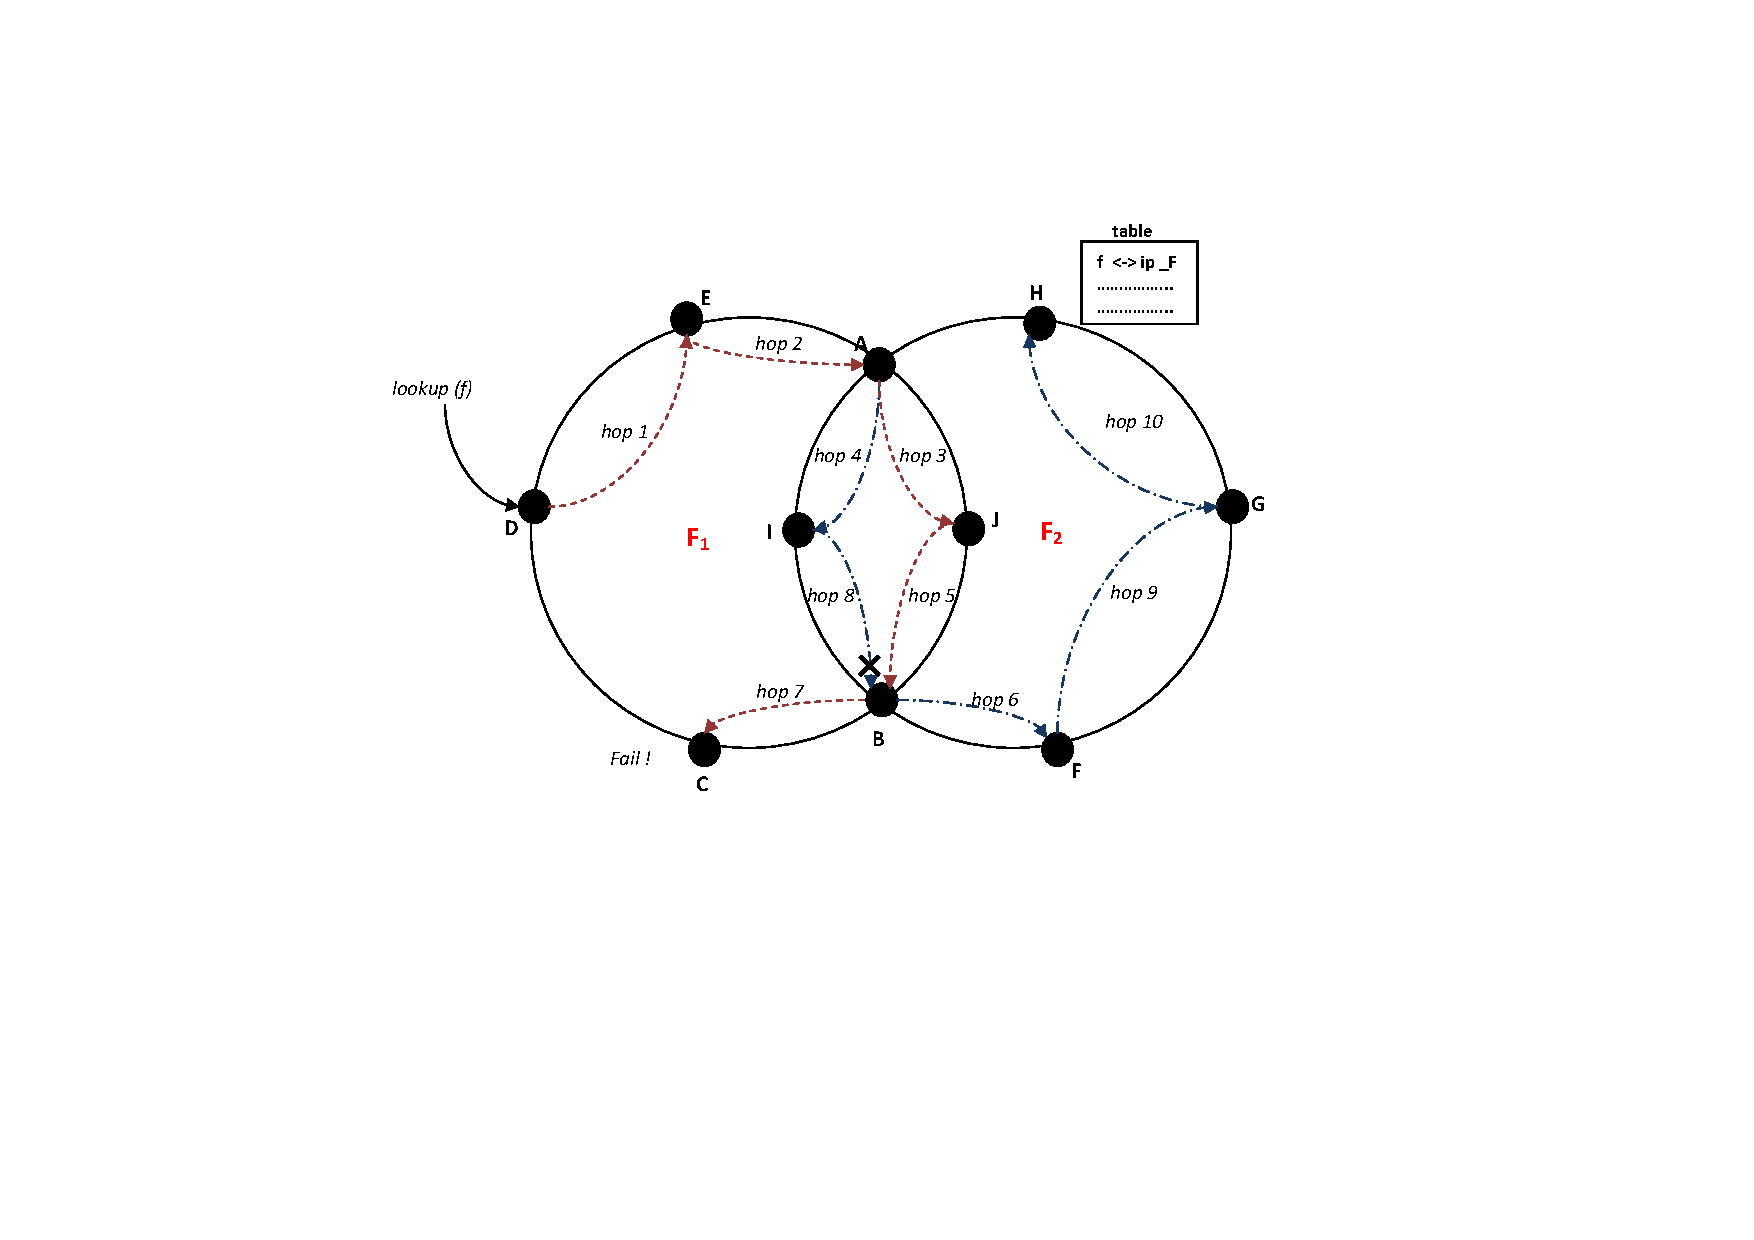
\includegraphics[width=1\linewidth]{fig/figure_example.pdf} \up{4}
  \end{center}
  \up{5}\caption{Multi-floor routing example \label{fig:multiFloorExample}}
\end{figure}




\up{4}\subsection{An example} \up{2}
%
We illustrate the Babelchord protocol by giving an example of a simple
two floors overlay topology and multi-floor lookup
routing. Figure~\ref{fig:multiFloorExample} shows a topology made of
two floors \verbi{F1} and \verbi{F2}. Nodes are depicted by capital
letters, \ie\ \verbi{A,B,..I}, and \verbi{J}.  Assume that every node
offers a single resource, \ie\ \verbi{a,b,...,i}, and \verbi{j}. The
two Babelchord floors intersect via two synapses nodes \verbi{A} and
\verbi{B}. Hops are labeled by an integer \verbi{i} denoting a global
time of arrival on a given node. Since intra-floor routing is
performed as in Chord, fingers and hand tables are hence omitted. For
graphical purposes, routing in the first floor moves clockwise, while
in the second floor moves anticlockwise. For
clarity, % Also for the sake of clarity,
we omit to hash nodes and resources via the two different hash
functions.

A \verbi{lookup(f)} is received by node \verbi{D} on floor \verbi{F1};
the intra-floor routing (hops \verbi{1} and \verbi{2}) goes to
\verbi{E} and \verbi{A} (the synapse) that, in turn, will trigger an
inter-floor routing on floor \verbi{F2} (hop \verbi{4}). The routings
proceed in parallel on both floors passing by nodes \verbi{I},
\verbi{J}, and \verbi{B} (hops \verbi{3,4,5} and \verbi{8},
respectively).

Since node \verbi{B} is the second synapse, when it receives the
\verbi{lookup(f)} by hop \verbi{8} on floor \verbi{F2}, it will not
forward it since it already saw the lookup triggered on \verbi{F1}.
In the meantime, the two lookups will continue their route to nodes
\verbi{C} (routing failure on floor \verbi{F1}), on nodes \verbi{F,G},
and finally terminate on node \verbi{H} hosting the value
\verbi{ip\_F} offering the resource \verbi{f}.




\begin{figure*}[!t]
{\scriptsize
\begin{alltt}
\textrm{\textbf{Node's Data structures}\medskip}
f(-)      \(\stackrel{de\!f}{=}\) hash(f)(-) \textrm{with} hash:int->Sha1\hfill{\rm the hash function f (small notation abuse)}
tag       \(\stackrel{de\!f}{=}\) (int)\(\sp{*}\)\hfill{\rm the list of all unique tags identifying a babelchord packet}
res       \(\stackrel{de\!f}{=}\) (r)\(\sp{*}\)\hfill{\rm the list of all resources offered by the current node}
table     \(\stackrel{de\!f}{=}\) (r,(ip)\(\sp{*}\))\(\sp{*}\)\hfill{\rm the associative array of resource-peers offering that resource}
succ      \(\stackrel{de\!f}{=}\) (f,ip)\(\sp{*}\)\hfill{\rm the associative array of successors at floor f}
pred      \(\stackrel{de\!f}{=}\) (f,ip)\(\sp{*}\)\hfill{\rm the associative array of predecessors at floor f}
fingers   \(\stackrel{de\!f}{=}\) [ip] \hfill{\rm array of ip addresses}
hands     \(\stackrel{de\!f}{=}\) (f,fingers)\(\sp{*}\)\hfill{\rm the associative array of fingers at floor f}
hotpeers  \(\stackrel{de\!f}{=}\) (ip,(f)\(\sp{*}\))\(\sp{*}\)\hfill{\rm the associative array of hot peers view by different floors}
hotfloors \(\stackrel{de\!f}{=}\) (f,(ip)\(\sp{*}\))\(\sp{*}\)\hfill{\rm the associative array of hot floors inhabited by different peers}
\end{alltt}} \up{5}
\caption{Node's data structures \label{fig:data}}
\end{figure*}
%
\begin{figure*}[!t]
{\scriptsize
\begin{alltt}
\textrm{\textbf{The Babelchord's protocol}}
\AL \textbf{on receipt of} LOOKUP(r) \textbf{from} ip \textbf{do}\alglabel{alg:lookupbegin}\hfill{\rm looking for nodes hosting resource r}
\AL   t = new_tag(ip);\hfill{\rm new unique tag for this lookup}
\AL   this.insert_tag(t); \hfill{\rm insert tag into the tag list}
\AL   \textbf{send} FINDSUCC(t,f,r,ip) \textbf{to} this.ip; \alglabel{alg:lookupend}\hfill{\rm send findsucc to itself}
\AL   \textbf{receive} FOUND(f,ip2) from ip3\hfill{\rm wait for the Babelchord routing}
\AL   \textbf{if} ping(ip2) \hfill{\rm test the aliveness of ip2}
\AL     this.update_hotpeers(ip2,f);\hfill{\rm update the hot peer list with ip2 at floor f}
\AL     this.update_hotfloors(f,ip2);\hfill{\rm update the hot floor list with f signaled by ip2}
\AL     \textbf{return} lookup_table(ip2,r);\hfill{\rm remote table lookup on ip2; return the list of ips offering the resource r}

\AL \textbf{on receipt of} FINDSUCC(t,f,r,ip) \textbf{from} ip2 \alglabel{alg:findsuccbegin}\hfill{\rm find the successor of ip}
\AL   \textbf{if} t = {join} \hfill{\rm join a floor}
\AL     \textbf{if} f(r)\( \in \)(f(this.ip),f(this.get_succ(f))]\hfill{\rm as in Chord}
\AL       \textbf{send} FOUND(f,this.get_succ(f)) \textbf{to} ip;\hfill{\rm found the successor of ip}
\AL     \textbf{else}
\AL       ip3 = this.closest_preceding_node(f,r); \hfill{\rm internal chord routing}
\AL       \textbf{send} FINDSUCC(t,f,r,ip) \textbf{to} ip3;\hfill{\rm send to the next hop}
\AL   \textbf{else if} not(this.in_tag(t)) \hfill{\rm lookup not processed}
\AL     this.push_tag(t); \hfill{\rm mark as ``already processed''}
\AL     \textbf{for all} f\( \in \)this.dom_hands() \textbf{do}\hfill{\rm for all floors of current node}
\AL       \textbf{if} f(r)\( \in \)(f(this.ip),f(this.get_succ(f))]\hfill{\rm test if arrived, as in Chord}
\AL         \textbf{send} FOUND(f,this.get_succ(f)) \textbf{to} ip;\hfill{\rm found a node hosting an entry for r}
\AL         \textbf{exit forall};\hfill{\rm stop the routing: ``game over''}
\AL       \textbf{else}
\AL         ip4 = this.closest_preceding_node(f,r); \hfill{\rm internal chord routing}
\AL         \textbf{send} FINDSUCC(t,f,r,ip) \textbf{to} ip4;\alglabel{alg:findsuccend}\hfill{\rm send findsucc to the next hop}

\textrm{\textbf{Auxiliary functions}}
\AL closest_preceding_node(f,r)\hfill{\rm internal function as in Chord}
\AL   \textbf{for} i = m \textbf{downto} 1 \textbf{do}\hfill{\rm for all fingers of floor f}
\AL     \textbf{if} this.lookup_hands(f)[i] \(\in\) (f(this.ip),f(r))\hfill{\rm testing the hand table as in Chord}
\AL       \textbf{return} this.lookup_hands(f)[i];\hfill{\rm return the finger of floor f}
\AL   \textbf{return} this.ip;\hfill{\rm return the current node ip}
\end{alltt}} \up{5}
\caption{Pseudocode for multi-floor resource lookup \label{fig:lookup}}
\end{figure*}




\up{2}\section{Babelchord's protocol}
%
\up{2}\subsection{Overview}\up{2}
%
In this section, we present the details of the algorithms building a
BabelChord network. First, we focus on the data structures used, \ie,
how Chord's data structures are extended to support multi-floor
architectures and protocols. Then, in Section~\ref{ssec:lookup}, we
give the main part of the protocol, \ie, the lookup within a
BabelChord network. Finally, in Section~\ref{ssec:tower}, we give an
idea of how peers can negotiate the creation of new rings and the
insertion of some node. Recall that the word \emph{floor} refers to
one Chord ring. Both words designate the same object.

\up{2}\subsection{Data structures for every peer}\up{2}
%
The structures used are detailed in Figure~\ref{fig:data}. Let
\verbi{f} represents both the identifier of a floor and, with a slight
abuse of notation, the hash function \verbi{hash(f)(-)} used at this
floor (we assume a distinct cryptographic hash function for each
floor).
%% one distinct function for each
%% floor), where \verbi{hash} is an higher-order function generating hash
%% functions (of the SHA* family).
The \verbi{tag} structure is a list of unique identifiers of
Babelchord requests, serving the \emph{cut-over} strategy. The
\verbi{res} structure represents the set of resources offered by a
single peer, while the \verbi{table} structure is the part of the hash
table the peer manages, containing the associative array of resource
keys and IP-addresses providing these resources. Every peer
contributes actively to routing through its \verbi{table} and to
resource exchange through the resources declared in \verbi{res}.  The
\verbi{succ}, \verbi{pred}, and \verbi{hands} structures contain
predecessor, successor and finger information for every floor a node
belongs to. Finally, \verbi{hotpeers} and \verbi{hotfloors} contain
information collected through lookups about peers for potential
collaborations and floors for potential participation.


\begin{figure*}[!th]
{\scriptsize
\begin{alltt}\NA
\AL \textbf{on receipt of} JOIN(f) \textbf{from} ip\hfill{\rm current peer invited by ip to join f}
\AL   \textbf{if} this.good_deal(f,ip)\hfill{\rm the invitation is a ``good deal'' (strategy left to implementers)}
\AL     this.add_hands(f,\(\bot\));\hfill{\rm add floor f to the hands associative array}
\AL     this.add_succ(f,\(\bot\));\hfill{\rm add a successor for floor f to the successor associative array}
\AL     this.add_pred(f,\(\bot\));\hfill{\rm add a successor for floor f to the successor associative array}
\AL     \textbf{send} FINDSUCC(join,f,this.ip,this.ip) to ip;\hfill {\rm find my successor}
\AL     \textbf{receive} FOUND(f,ip2) \textbf{from} ip3;\hfill{\rm receiving the response}
\AL     this.reassign_succ(f,ip2);\hfill{\rm reassign ip3 as my successor at floor f}
\AL     \textbf{for all} r\( \in \)res \textbf{do}\hfill{\rm for all the resources offered by the current node}
\AL       \textbf{send} FINDSUCC(join,f,r,this.ip) to ip;\hfill {\rm find the node hosting the table entry for r}
\AL       \textbf{receive} FOUND(f,ipr) \textbf{from} ip4;\hfill{\rm waiting for response}
\AL       \textbf{if} ping(ipr) \hfill{\rm test the aliveness of ipr}
\AL         update_table(ipr,r,this.ip);\hfill{\rm the table stored on ipr is updated with the new bind for r with this.ip}

\AL \textbf{on receipt of} JOINREQ(f) \textbf{from} ip\hfill{\rm the current peer ask to ip to join the floor f}
\AL   \textbf{if} this.good_deal(f,ip)\hfill{\rm accept ip at floor f is a ``good deal'' (strategy left to implementers)}
\AL     \textbf{send} JOIN(f) to ip;\hfill{\rm accept ip at floor f}
\end{alltt}} \up{4}
\caption{Pseudocode for join and join request \label{fig:join}}
\end{figure*}




\begin{figure*}[!th]
{\scriptsize
\begin{alltt}
\textrm{\textbf{Runned periodically, in order to make some inter-floor business}}\NA

\textrm{\textbf{Join a hot floor (increase local, i.e. node, connectivity)}}
\AL join_new_floor()
\AL   \textbf{select} f\( \in \)(this.dom_hotfloors() \(\setminus\) this.dom_hands());\hfill{\rm select one floor to join (strategy left free)}
\AL   \textbf{select} ip\( \in \)this.select_node(f);\hfill{\rm select one node of f to send a join request}
\AL     \textbf{send} JOINREQ(f) \textbf{to} ip;\hfill{\rm send an invitation to ip to join floor f}

\textrm{\textbf{Invite an hot node to a randomly chosen floor (increase semilocal, i.e. floor, connectivity)}}
\AL  invite_new_node()
\AL    \textbf{select}  f\( \in \)this.dom_hands();\hfill{\rm select one floor to invite a node (strategy left free to impl.)}
\AL    \textbf{select} ip\( \in \)this.dom_hotpeers();\hfill{\rm select one hot node to invite (strategy left free to impl.)}
\AL    \textbf{if} this.good_deal(f,ip)\hfill{\rm the invitation is a ``good deal'' (strategy left to implementers)}
\AL      \textbf{send} JOIN(f) \textbf{to} ip;\hfill{\rm send an invitation to ip to join floor f}

\textrm{\textbf{Create a new floor from scratch (increase global, i.e. BabelChord, connectivity)}}
\AL  create_new_floor()
\AL    f = new_floor(ip) ;\hfill{\rm a new floor function is created}
\AL    this.add_hands(f,\(\bot\));\hfill{\rm \(\bot\) is the new floor}
\AL    this.add_pred(f,\(\bot\));\hfill{\rm \(\bot\) is the predecessor}
\AL    this.add_succ(f,ip);\hfill{\rm ip itself is the successor}
\end{alltt}} \up{6}
  \caption{Pseudocode for negotiating new joins\label{fig:business}}
\end{figure*}


\up{2}\subsection{The lookup protocol \label{ssec:lookup}}\up{2}
%
The multi-floor lookup is illustrated in
Figure~\ref{fig:lookup}. Lines $1.01$ to $1.04$ initiate a
\verbi{lookup} on a resource \verbi{r}.

After creating a new unique tag for this request, the current node
initiates the lookup by sending a \verbi{FINDSUCC} message to itself,
and waits for the response, \ie, a \verbi{FOUND} message specifying
the IP-address of a node storing the sought key. On receipt of a
\verbi{FINDSUCC} message (Line $1.10$), the current node distincts two
types of messages:
%
\up{2}\paragraph*{Join routing (Lines 1.12-1.16).} When the first
element of the message is a \verbi{join} tag, it means, as we will
detail later, that the lookup serves a join purpose. The request is
then routed as in a simple Chord \verbi{join}, and corresponds to the
routing process of either a resource registration or a peer
insertion. Note that when the requested \verbi{id} falls between the
current node and its successor \verbi{succ}, the node targeted by the
routing is \verbi{succ}. A \verbi{FOUND} message is returned to the
initiator of the routing \verbi{ip} at Line $1.13$.
%
\up{2}\paragraph*{Resource lookup routing (Lines 1.18-1.25).} If the
first element of the message is a numeric tag, it means that the
message is part of a resource lookup request. The message can then be
routed in several rings the current node belongs to. First, the tag of
the request is checked (Lines $1.17$-$1.18$). If the request was
already processed, it is simply ignored, implementing the
\emph{cut-over} strategy. Otherwise, the request tag is saved in order
to avoid routing the same request several times. Note that, the
requests are routed according to every floor a node belongs to.
% It may be envisioned that the request may be routed to only a subset
% of floors, dynamically chosen by the current node, according to a
% local policy.
When the routing reaches its destination on a given floor, a
\verbi{FOUND} message containing the address of the node storing the
information on the requested resource, is sent back to the initiator
of the lookup. On receipt of \verbi{FOUND} (Lines $1.05$-$1.09$), the
initiator checks the aliveness of the node \verbi{ip} returned and
rewards it locally by updating the reputation of \verbi{ip} in its hot
peer and hot floor lists. Finally, it remotely reads the values wanted
(Line $1.09$). Lines $1.26$-$1.30$ detail one local routing step
(finding the closest preceding node among my fingers) for the next
step.  This part is very similar to the Chord local routing step, but
integrating the floor information.


\up{2}\subsection{New floor creation (tower building) \label{ssec:tower}}\up{2}
%
Figures~\ref{fig:join} and~\ref{fig:business} show the creation of
new floors:
% We first give the details of the receipt of two building block
% messages serving the creation of new floors:
\verbi{JOIN} and \verbi{JOINREQ}. Lines $2.01$ to $2.13$ detail the
reception of a \verbi{JOIN(f)} message which is an invitation to join
floor \verbi{f} from a node \verbi{ip}, already member of
\verbi{f}. On receipt, the node decides whether it is a \emph{good
  deal} or not to join \verbi{f} %according to some local information
(Line $2.02$). If this is the case, the current node initiates its
join to \verbi{f} by sending a \verbi{FINDSUCC} message to \verbi{ip}
and waits for its information required to belong to \verbi{f}, namely,
its \verbi{successor}. On receipt, the current node registers its
resources \verbi{res} into the floor %, one by one
(Lines $2.09$-$2.13$). Lines $2.14$ to $2.16$ detail the receipt of
the \verbi{JOINREQ(f)} message, used to request an invitation. On
receipt, the node evaluates the advantages and drawbacks of accepting
a new node at floor \verbi{f} and sends an invitation in the case of a
positive evaluation.

Through Figure~\ref{fig:business}, we show the pseudocode for
proposing, negotiating, and accepting new
connections. % in BabelChord.
The following functions are periodically triggered:
\verbi{join\_new\_floor} (Lines $3.01$ to $3.04$) selects one floor
(among the hot floors list) and requests an invitation to one node of
this floor. \verbi{invite\_new\_node} (Lines $3.05$ to $3.09$) selects
a node to invite at a given floor (this node must reach the
\verbi{good\_deal} requirements). \verbi{create\_new\_floor} (Lines
$3.10$ to $3.14$) initiate the creation of a new floor for future
invitations.

Note that any strategy for choosing nodes and floors can be
implemented. Strategies may include evaluating nodes and floors
according to performance, resources provided, presence rate, etc.


\up{2}\section{Simulation results}\up{2}
%
To better capture its relevance, we have conducted some simulations of
the BabelChord approach. The simulator, written in Python, works in
two phases. First, a Babelchord topology is created, with the
following properties: (i) a fixed network size (the number of nodes)
$N$, (ii) a fixed number of floors denoted $F$, (iii) a fixed global
\emph{connectivity}, \ie, the number of floors each node belongs to,
denoted by $C$. As a consequence: (i) The nodes are uniformly
dispatched among the floors, \ie, each node belongs to $C$ floors
uniformly chosen among the set of floors. (ii) Each resource provided
by nodes is present at $C$ floors. (iii) The average lookup length
within one given floor is $\log((N \times C)/F)/2$.

In a second time, the simulator computes the number of hops required
to reach one of the node storing one of the key of a particular
resource. Results are given for different values of $N$, $F$, and
$C$. Figure~\ref{fig:simu1} gives the results for $C{=}2$ and
$F{=}10,50,100$. Note that, in this case, the size of the routing
table is in $O(\log((N \times C)/ F)){<}O(\log(N))$. The curves
clearly demonstrates the logarithmic behavior of such an
architecture, even if the average number of hops remains slightly
above the Chord reference ($\log(N)/2 $). Note also that, the curves
suggest that when the ratio $C/F$ decreases, the lookup length
increases. This statement is rather intuitive: at each multi-floor
routing step, the relative number of floors reached by a request
depends on this ratio. Figure~\ref{fig:simu1} also presents the same
experiments with $C{=}5$. As expected, the lookup length is slightly
reduced compared to the results with $C{=}2$. Finally,
Figure~\ref{fig:bab_last} shows the number of synapses vs. the lookup
success rate. Only 5\% of synapses made of 2 (resp. 3, 5, 10) floors
connections in the whole node population is enough to achieve more
than 50\% (resp. 60\%, 80\%, 95\%) of exhaustive lookups in the
Babelchord network.
%
\begin{figure}[!htb]
  %%%% MERGER AVEC UN EDITEUR ALA GIMP LE DEUX FIGURES
   %\up{2}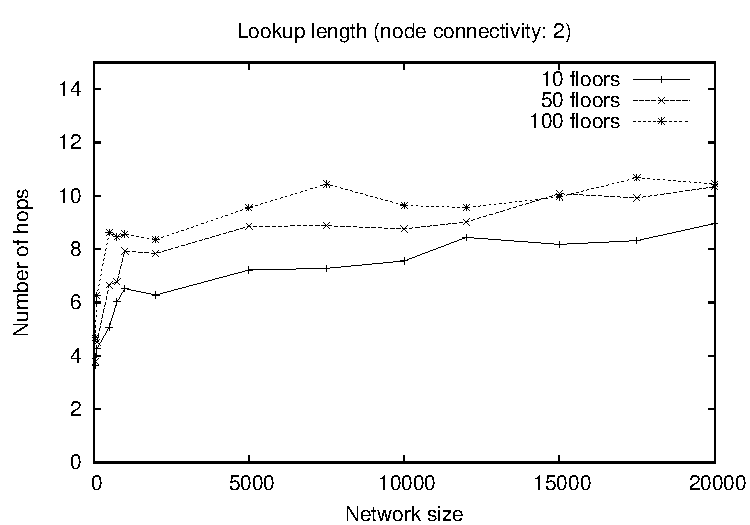
\includegraphics[width=\linewidth]{fig/bab_c2}\up{15}\\
   \up{2.05}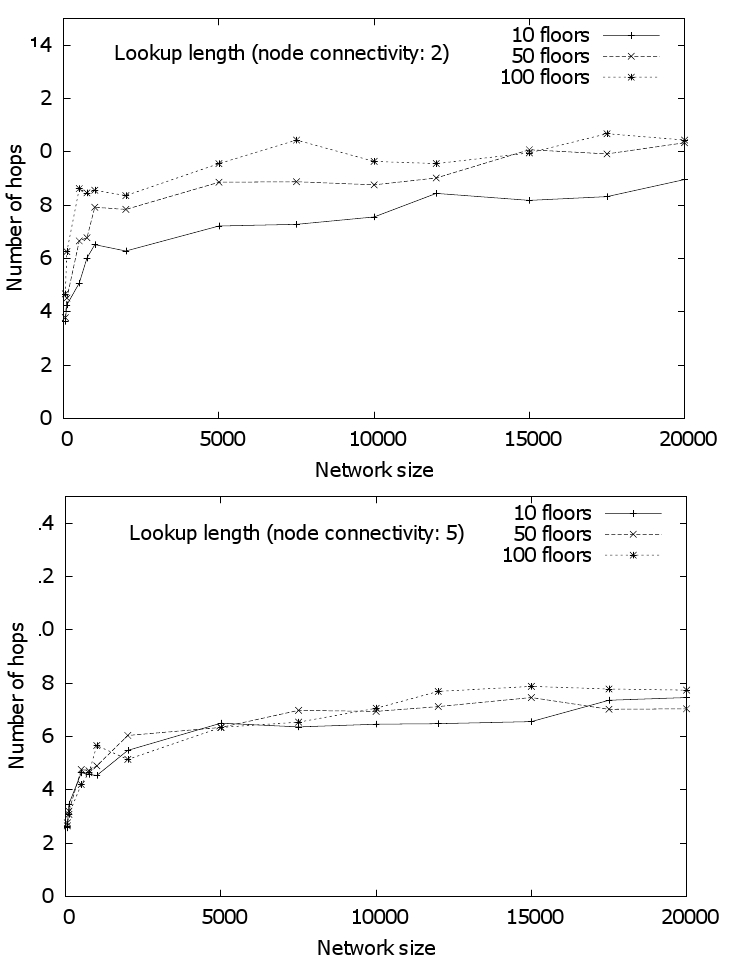
\includegraphics[width=\linewidth]{fig/C2andC5.jpg} \up{2}
   \up{7}\caption{Lookup length, $C{=}2$ and $C{=}5$ \label{fig:simu1}}
\end{figure}
%
% \begin{figure}[!htb]
%   \up{2}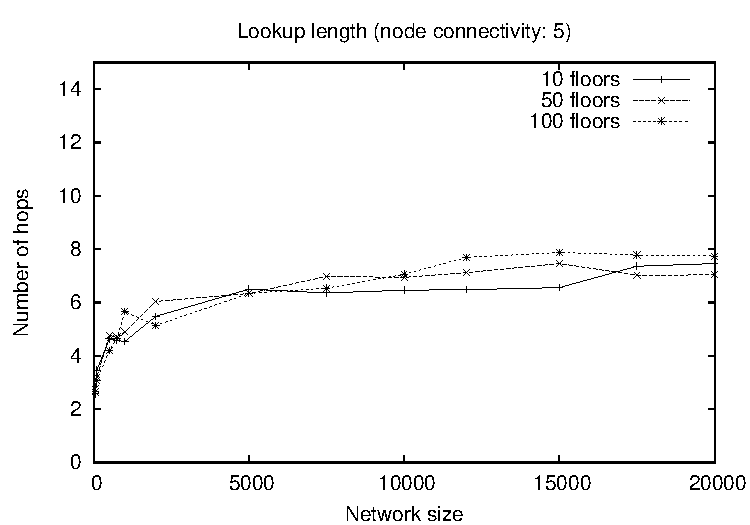
\includegraphics[width=\linewidth]{fig/bab_c5} \up{2}
%   \caption{Lookup length, $C{=}5$\label{fig:simu2}}
% \end{figure}

\up{5}
\begin{figure}[!htb]
  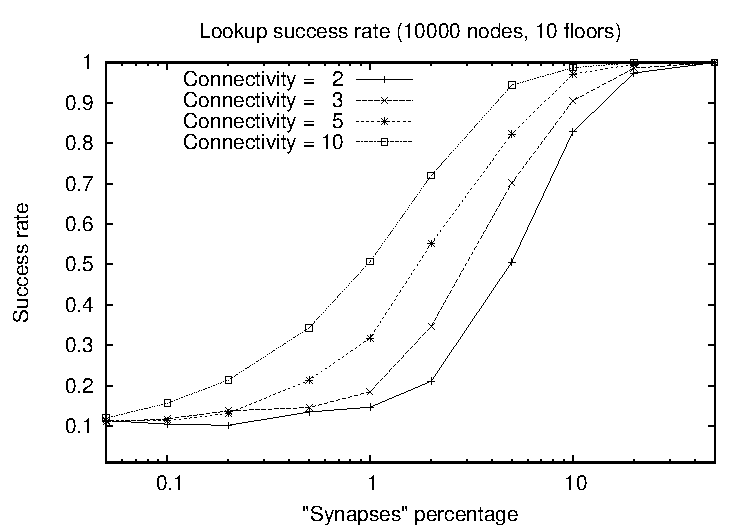
\includegraphics[width=\linewidth]{fig/bab_last}\up{2}
  \up{5}\caption{Exhaustiveness, $N{=}10000$ \label{fig:bab_last}}
\end{figure}


\up{5}\section{Conclusions}\up{2}
%
We have presented Babelchord, a social tower of Chord-based
DHTs. Babelchord proposes a simple method for aggregating DHTs
(floors) based on intersection nodes, called synapses. Synapses can be
created by keeping a list of hot peers and floors and by negotiating
between nodes following some ``good deal'' criterion, left free to
every node implementation. Babelchord proposes to aggregate small
\emph{structured} overlay networks in an \emph{unstructured} fashion
and is an alternative approach to rigid hierarchical peer-to-peer
systems.

Simulation confirms that Babelchord scales well with the number of
nodes and floors, exhibiting logarithmic behavior. It illustrates the
relevance of connecting smaller structured network in an unstructured
fashion, within which each node is free to select its neighbors
according to its own policy. From a networking point of view, the
rationale is simple: \emph{the more synapses we have, the more
  exhaustive and fast the routing is!}

% We believe that Babelchord can be fruitfully applied in Internet
% applications dealing with software and hardware barriers or in fully
% distributed social-network applications.  , or in large-scale brain
% model and simulation experiments.

%% EVENTUALLY USE THIS IN SMALL
{\small
\begin{thebibliography}{10}

\bibitem{CCL08}
R.~Chand, M.~Cosnard, and L.~Liquori.
\newblock {Powerful resource discovery for Arigatoni overlay network}.
\newblock {\em Future Generation Computer Systems}, 1(21):31--38, 2008.

\bibitem{Datta}
A.~Datta and K.~Aberer.
\newblock The challenges of merging two similar structured overlays: {A} tale
  of two networks.
\newblock In {\em Proc. of IWSOS}, 2006.

\bibitem{Biersack}
L.~G. Erice, E.~W. Biersack, K.~W. Ross, P.~A. Felber, and G.~U. Keller.
\newblock Hierarchical p2p systems.
\newblock In {\em Proc. of Euro-Par}, 2003.

\bibitem{Biersack2}
L.~G. Erice, K.~W. Ross, E.~W. Biersack, Pascal~A. Felber, and G.~U. K.
\newblock Topology-centric look-up service.
\newblock In {\em Proc. of NGC}, 2003.

\bibitem{LC07b}
L.~Liquori and M.~Cosnard.
\newblock {Logical Networks: Towards Foundations for Programmable Overlay
  Networks and Overlay Computing Systems}.
\newblock In {\em TGC}, volume 4912 of {\em LNCS}, pages 90--107. Springer,
  2007.

\bibitem{CAN}
S.~Ratnasamy, P.~Francis, M.~Handley, R.~Karp, and S.~Shenker.
\newblock {A Scalable Content-Adressable Network}.
\newblock In {\em ACM SIGCOMM}, 2001.

\bibitem{Haridi}
T.~M. Shafaat, A.~Ghodsi, and S.~Haridi.
\newblock Handling network partitions and mergers in structured overlay
  networks.
\newblock In {\em Proc. of P2P}, pages 132--139. IEEE Computer Society, 2007.

\bibitem{Chord}
I.~Stoica, R.~Morris, D.~Karger, M.~Kaashoek, and H.~Balakrishnan.
\newblock {Chord: A Scalable Peer-to-Peer Lookup service for Internet
  Applications.}
\newblock In {\em ACM SIGCOMM}, pages 149--160, 2001.

%\bibitem{ECAN}
%Z.~Xu and Z.~Zhang.
%\newblock {Building Low-Maintenance Expressways for P2P Systems}.
%\newblock Technical report, Hewlett-Packard Labs, 2002.

\bibitem{brocade}
B.~Y. Zhao, Y.~Duan, L.~Huang, A.~D. Joseph, and J.~D. Kubiatowicz.
\newblock {Brocade: Landmark Routing on Overlay Networks}.
\newblock In {\em IPTPS 2002}.

\end{thebibliography}
}
\end{document}


% \begin{theorem}
%   With high probability, the number of nodes that must be contacted
%   to find a successor on a $N_1\times...\times N_k$-node network of
%   $k$ floors is $min(O(log(N_1)),...,O(log(N_k))$
% \end{theorem}

% \begin{theorem}
%   With high probability, the number of nodes that must be contacted
%   to (or to route back a success notification) on a
%   $N_1\times...\times N_k$-node network of $k$ floors is
%   $min(O(log(N_1)),...,O(log(N_k))$
% \end{theorem}

% \begin{theorem}
%   With high probability, and without (respectively with) Game-over
%   cut routing, the number of messages exchanged to find a successor
%   (or to route back a success notification) in a $N_1\times...\times
%   N_k$-node network of $k$ floors is $\sum_{i=1..k}O(log(N_i))$
%   (respectively $M \le \sum_{i=1..k}O(log(N_i))$).
% \end{theorem}



CONJECTURE

- With high probability and with time->infinity, an infinite number of
chord will "simulate" a fully connected graph, with routing complexity
-->_infty O(1), as in a plain array.


\section{Distributed Construction Mechanism}

At a given time, and within the default overlay (level $0$), a peer
$P$, which observed that a lot of its requests are satisfied by
another peer $Q$ may contact $Q$ for a possible collaboration. On
receipt, $Q$, which is a member of at least one overlay at level $1$,
enters in a negociation phase intended to decide whether $P$ may be a
neighbor of $Q$ on level $1$. This decision may be done on several
aspects, like \emph{capacities}, \emph{trust}, \emph{content},
etc. $Q$ can asks its neighbors on level $1$ in order to obtain a
consensus on a possible membership of $P$. If $P$ has no membership at
level $1$, $P$ and $Q$ may initiate a new ring.

This mechanism can be easily extended to an arbitrary number of levels
(just replace $0$ by $m$ and $1$ by $m+1$. A peer may be the member of
several rings of the same level.

An $m$-ring (ring at level $m$) is always a refinement of an $m-1$
ring in which members consider the $m$ ring as more \emph{powerful}
(in their own point of view).

\section{Complexities}

The number of members in a ring may be limited. For instance, consider
that at level $1$, the members of a ring decide that no more than
$\log(n)$ peers should enter their ring, $n$ being the number of peers
at level $0$. As a consequence, routing table size and lookup length
at level $1$ will be $\log(log(n))$. If we apply the same rule at each
level, when the number of levels tends to infinity, the routing table
size and lookup length will be $\log^*(n)$, which increases very
(very) slowly.

In a more general point of view, we can consider that the maximum
number of members $N_m$ of a $m$-ring is always a function of $N_{m-1}$:

$$
N_m = f(N_{m-1})
$$

This function can be $\log()$ or the $\sqrt()$. Now, the number of
rings in which a peer acts at a given level may also be
limited. Finally, we have to find the right trade-off between the
number of levels, the size of rings at each level and the number of
rings a peer may belong to at a same level. (Thinking on this part...)



